\chapter{Extending Local Feature Based Models of SV Detection in a Discriminative Machine Learning Framework}\label{chap_crf}

\todo{clarify states for Brian, see if I have data comparing states}
\todo{talk about Zinfandel}

In the formulation of a general algorithmic framework for SV prediction in MapReduce that we described in Chapter~\ref{chap_framework}, a crucial step is the computation of a set of features for each of the small, non-overlapping windows with which we tiled the genome reference. In the implementation of Cloudbreak described in Chapter~\ref{chap_cloudbreak_impl}, these features were the parameters which are estimated by fitting a GMM to the distribution of insert sizes that span that location. However, in general the nature of these features are purposefully not specified in the algorithmic framework to allow flexibility in the nature of the applications that it could potentially be used to build.

Given a set of arbitrary features that encode information about a set of loci that are connected in a sequence, a natural approach is to apply techniques from machine learning to identify regions of interest in that sequence, rather than the heuristics and noise reduction techniques from signal processing that are used in the Cloudbreak implementation described in Chapter \ref{chap_cloudbreak_impl}. In this chapter we will reformulate the problem as a sequence labeling task, discuss possible machine learning frameworks that could be used to solve it, explore the ways in which features can be engineered to integrate multiple signals of SVs, and show that it is possible to achieve modest but positive improvements using conditional random fields, a discriminative machine learning technique.

\section{Related Work}

Discriminative machine learning techniques have been applied to SV detection in the tools forestSV~\cite{Michaelson:2012fj} and SVM$^2$~\cite{Chiara:2012ey}. SVM$^2$ computes a set of statistics based on differences between the coverage and insert size distributions observed at nearby locations on the genome. If the statistics pass a set of coarse filtering rules, they are used as features for a support vector machine (SVM) classifier that the authors trained on a set of simulated short insertion and deletions. forestSV trained a Random Forest classifier~\cite{breiman2001} to detect deletions and duplications based on validated and false positive predictions from many samples in the 1000 Genomes Project data set. Their tool is based upon computing features for a sliding window moving across the genome, as well as for the flanking regions of that window. The authors demonstrated that it was possible to combine disparate signals by including features that were based on read depth as well as discordant read pair mappings in their feature set. The forestSV algorithm was similar to Cloudbreak in that the classifier made calls at each window, and a postprocessing function then merged windows classified with the same label into variant calls. Both of these methods demonstrate innovative ways of learning from existing data, and integrating read pair and split read based signals. However, neither of these tools use machine learning techniques that take into account the sequential nature of the data; the classifiers are run independently on each candidate variant location (in the case of SVM$^2$) or window (in the case of forestSV), and the labels that are assigned in each invocation of the classifier do not affect the neighboring regions. We will show that by treating the problem as a sequence labeling task, it is possible to take advantage of learning techniques that operate on the entire sequence of observations at once.

\section{SV Detection as a Sequence Labeling Problem}

In our MapReduce algorithmic framework, the features computed at each window are transformed into variant calls by a function that examines the features along each chromosome of the reference sequentially and identifies contiguous blocks of regions with features values that combine to coherently indicate the presence of a variant. This part of the process, which we named the \textsc{Postprocess} function in Algorithm \ref{cb_algo}, can be thought of as a sequence labeling problem based on a series of observation features. To take the example of deletion detection, we could define two labels: ``Deletion'' if the window participates in a deletion variant, and ``No Deletion'' if it does not. More formally, we can let $Y_i$ be the label at genomic window $i$, where $1 \le i \le n$ and $n$ is the number of windows in the chromosome. If we similarly name the features for genomic window $i$ $X_i$, we can then refer to the entire sequence of labels and features as $Y$ and $X$, respectively.

The goal of the \textsc{Postprocess} function can be broken down into two parts: first, to assign a label to each window in the reference sequence, and second, to consolidate neighboring windows with the same label into variant calls which affect larger regions. Analyzing the implementation of Cloudbreak described in Chapter \ref{chap_cloudbreak_impl} in this model, we used a simple linear threshold on the likelihood ratio of the insert size data to label each window, and then consolidated neighboring windows with hand-tuned rules such as the median filter and restriction on the estimated mean of the second GMM component. These latter rules were made necessary by the noisy nature of the data and the simplicity of the window-labeling procedure. However, if we had a completely accurate window-labeling procedure, we could remove much of the complexity of the consolidation step. Since real world data is noisy the best that we can do is to try to find the most likely sequence of labels given the observed data:

\[ \argmax_Y P(Y|X) \]


\section{Graphical Models for Sequence Labeling}

To achieve the goal of a more principled and more accurate window-labeling procedure we would need to be able to take into account information from multiple features, as well as the labels of nearby windows. In other words, the label of each window should be dependent not only on the observed features at that window but also on the labels of other windows nearby. Probabilistic graphical models provide a useful framework for defining and learning models that describe these types of dependencies. One class of graphical model that has been used extensively for sequence labeling tasks in bioinformatics are Hidden Markov Models (HMMs). HMMs model sequence labeling problems by assuming that the observations at each point are dependent on a hidden state, and that the state at a given time is dependent on the state at the previous time step. If one creates an HMM such that the hidden states correspond to the labels of interest, the task of learning an HMM is equivalent to learning a probability distribution $P(Y_i|Y_{i-1})$ that describes the likelihood of moving from one state to another, and a distribution $P(X_i|Y_i)$ that gives the likelihood of seeing a particular observation given the true label at that time point, which can be modeled by a directed graphical network (Figure~\ref{graphical_model_hmm}). Therefore, HMMs are generative models that model the entire distribution over labels and observations, or the joint distribution $P(Y,X)$. One published CNV detection algorithm, Zinfandel~\cite{Shen:2011ku}, used an HMM to predict the presence of deletions and duplications. That algorithm used a feature set consisting of the read depth at each location and likelihood of the distribution of insert sizes given varying fixed potential sizes of deletions.

\begin{figure}
\centering
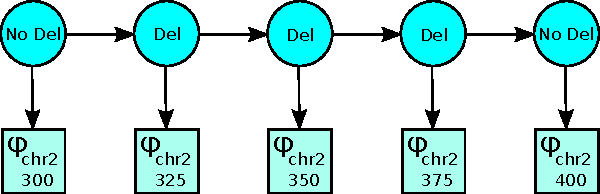
\includegraphics[width=.8\textwidth]{figures/graphical-model-1.pdf}
\caption[A Hidden Markov Model for the SV detection problem.]{A Hidden Markov Model for the SV detection problem.}
\label{graphical_model_hmm}
\end{figure}

One downside to modeling the joint distribution over features and labels is that what we are really interested is the conditional distribution $P(Y|X)$: given the observations, what is the most likely sequence of labels? Since $P(Y,X) = P(Y|X) * P(X)$, by training an HMM we are forced to learn $P(X)$, or the distribution over sequences of observations, even though it does not help us achieve our goal. A second drawback to HMMs, particularly in the proposed application of SV detection, is the fact that the model assumes that $P(X_i)$ is independent of $P(X_{i-1})$ given $Y_i$. In other words, observations drawn from the same state should all be independent. For the SV detection problem described here, this seems highly restrictive: for many features we might imagine, observations from two different genomic windows that are participating in the same deletion variant are likely to be much more similar than two windows that are participating in different deletion variants, even though they all share the label ``Deletion''. As the developers of Zinfandel noted, this required them to create a grid of ``Deletion'' and ``Deletion Flank'' states, with each row corresponding to a different size class of deletion variant.

Conditional random fields~\cite{Lafferty:2001:CRF:645530.655813} (CRFs) offer solutions to each of these drawbacks. In contrast to HMMs, CRFs are Markov Random Fields which can be represented by undirected graphical models. Because the model is undirected, it is possible to directly learn the conditional distribution $P(Y|X)$ from a set of training data. Training and inference of these models is tractable for simplified graphical structures; for our application we will use a \emph{linear chain CRF}, which mimics the structure of a sequence of observations and its labels (Figure~\ref{graphical_model_crf}). Furthermore, CRFs represent the factors that relate the observation sequence to the label node at position $i$ in the sequence in the graph through a log-linear model over a set of $k$ feature functions:

\[ \exp \left( \sum_k \theta_k f_k(y_i, y_{i-1}, X) \right) \]

This means that the feature functions for each position $i$ in the sequence can incorporate information from observations any point in the observation sequence. This removes the requirement that observations be independent from one another, and allows the consideration of features taken from neighboring observations, something that could be useful in our context of SV detection, where multiple small genomic windows are spanned by single reads and fragments.

\begin{figure}
\centering
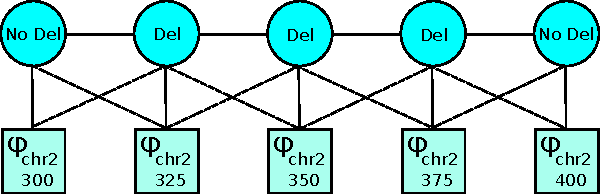
\includegraphics[width=.8\textwidth]{figures/graphical-model-2.pdf}
\caption[A linear chain Conditional Random Field model of the SV detection problem.]{A linear chain Conditional Random Field model of the SV detection problem. Label nodes can be connected by feature functions to any of the observations in the sequence.}
\label{graphical_model_crf}
\end{figure}

\section{Integrating Features with Conditional Random Fields}

We implemented a linear-chain conditional random field model to label genomic insertions and deletions. The model was developed using Factorie~\cite{mccallum09:factorie}. Factorie is a toolkit written in Scala that supports a wide variety of factor-graph based models, trainers, and tools, particularly for NLP tasks such as named entity recognition. Our Factorie-based implementation of a structural variation detection program consists of two parts: a modular and configurable set of code for data management of features defined along the genome, along with conversion of real-valued features into into binary binned feature values, and code to construct, train, and run inference on linear-chain CRF models. The code developed for this project was written in Scala and is available on GitHub at \url{http://github.com/cwhelan/svfactorie}. 

\section{Features for SV Detection}

As described in Chapter \ref{chap_background}, there are three main signals available for SV detection in short read sequencing data sets: those that come from read pairing information, those that come from read depth, and those that come from split reads. The creation of a discriminative machine learning framework as described above can be used with any arbitrary set of features. Therefore it is possible to create feature sets that combine information from all three SV detection signals and integrate them into this framework. In addition, we can model interactions between features and use those in our predictions. Finally, the arbitrary nature of the feature function allows us to incorporate prior knowledge about given genomic regions, including sequence annotations. We have constructed a feature set that includes all of these types of features, as described below:

\subsection{Read Pair Features}

Read pair features are those that are based upon the inferred insert sizes and orientations linking paired reads, as described previously. We use the following RP features:

\begin{itemize}

\item The three features generated by Cloudbreak and described in Chapter~\ref{chap_cloudbreak_impl}: the log likelihood ratio of the insert sizes observed at each window in the two-component GMM fit vs. the likelihood under the expected normal distribution for the sample; the estimated mean $\mu_2$ of the second component of the two-component GMM, and $\alpha$, the estimated weight of the second component in the two-component GMM.

\item Insert size change point features: in addition to the insert size calculations described in the Cloudbreak implementation, we also wanted to consider alternative features based on insert sizes. In particular, we wanted to test whether the addition of features that indicate whether a window represents a point at which the insert size distribution in a local surrounding region is changing would improve identification of variants. We compute such a score as follows: let $i$ be the index of a window in the genome, and $S_{i..j}$ be the list of observed insert sizes spanning the windows labeled $i$ through $j$. Now consider a local neighborhood of size $n$ which comprises the windows $i-\frac{n}{2},...,i,...,i+\frac{n}{2}$. Let $\Theta_{i..j}$ be model parameters that can be estimated from the distribution of insert sizes $S_{i..j}$, and $P(S_{i..j}|\Theta_{i..j})$ be the likelihood of observing $S_{i..j}$ under the model with parameters $\Theta$. We can calculate a change score for each window $i$ by examining the likelihood of the data in the halves of the neighborhood to the right and left of that window, by estimating $P(S_{i-\frac{n}{2}..i})$ and $P(S_{i+1..i+\frac{n}{2}})$. Simultaneously, we can perform the same estimates for all of the data in the neighborhood and compute $P(S_{i-\frac{n}{2}..i+\frac{n}{2}})$. The likelihood ratio between these two models:

\[ \frac{P(S_{i-\frac{n}{2}..i}) * P(S_{i+1..i+\frac{n}{2}})}{ P(S_{i-\frac{n}{2}..i+\frac{n}{2}})} \]

then serves as a score indicating the presence of a change between the segments to the left and right of point $i$. This has the advantage of being a parameter-free calculation, since parameters are re-estimated from each segment for each calculation. According to the Cloudbreak's model, it would be natural to estimate two component GMMs for each segment of insert size data. However, in practice we found that changes were well captured by the likelihood ratio score when only a single-component Gaussian is used for each segment, and so we have used that model for the sake of efficiency. We use a neighborhood size of 200 bp.

\end{itemize}

\subsection{Split-read features}

Split read signals are caused when a read overlaps a genome breakpoint, disrupting the full alignment of that read. If only simple variants are considered, such a scenario should reveal the exact location of the breakpoint. However, these are difficult to resolve in practice, because the algorithm must first identify potentially split reads from those that fail to align or partially align, and then align the two ends of the split read to the genome, potentially at large distances from one another. True split-read based SV detection methods use dynamic programming and heuristics to try to accomplish this; however, the difficulty of doing so with current read lengths means that they have low sensitivity (although very high specificity). Rather than conduct an exhaustive split read alignment search, we instead use indirect evidence of split reads that can be extracted from standard first-pass alignments:

\begin{itemize}
\item Soft clipping: When reads are aligned to the genome by short read mappers like BWA, they can in some cases be only partially aligned. In BWA, this occurs when a parameterized clipping penalty is less than the additional cost of aligning the rest of the read according to a Smith-Waterman dynamic programming alignment. Aligners refer to this "soft clipping", and flag the read with specific indicators when it occurs. Although there are other possible reasons for soft clipping (for example, the quality could fall at the end of the read, producing many erroneous mismatches with the reference), this could potentially be indicative of a structural variation breakpoint disrupting the read's alignment to the reference. For integration into the CRF feature set, we created a feature track that counts the number of times a soft clip occurred in each 25bp genomic window.

\item Singleton alignments: For paired end reads, sometimes only one read in the pair can be successfully aligned to the genome. These are referred to as "singleton" alignments. Potentially a singleton alignment could indicate that the other read in the pair contains a variant that prevented it from being aligned, and therefore that a breakpoint could lie somewhere within the distance of the insert size, or could have disrupted the alignment of the other read in the pair. We count the number of singleton alignments in each window. \todo{Visually inspecting the data, and looking at the trained weights in my model, this doesn't seem like a very useful feature in practice.}
\end{itemize}

\subsection{Read depth features}

The third major signals of structural variations from short-read sequencing data are related to read depth. In the context of deletions, one would expect to see fewer reads aligning to sections of the genome which have been deleted in the sample; if the deletion is 100\% represented in the sample and is homozygous, any reads aligning to that location must be incorrect alignments. In practice, coverage depth is affected by noise resulting from incorrect mappings and biases of the sequencing process (for example, the amount of GC content in a given fragment of DNA will affect its representation in the sequencing data set). 

\begin{itemize}
\item Coverage depth: As one feature, we calculate the average coverage depth of each base in each 25bp window.

\item Coverage change points: We applied the change point detection algorithm outlined in the previous section to identify windows at which the coverage changes. Although we experimented with different neighborhood sizes, we found that this was not a very valuable feature for breakpoint identification. For the results reported below, we used a neighborhood size of 600bp.

\item Coverage Drops: We speculated that for the specific case of deletion detection, the most informative coverage statistic might be one that indicates whether or not the coverage at a given window drops relative to its local neighborhood. Therefore, we compute for each window the drop in coverage depth from the mean coverage depth of the windows that lie in the surrounding 500bp.
\end{itemize}

\subsection{Genome annotations}

Finally, the ability to include arbitrary features in the model allows us to incorporate prior knowledge about the genome into our feature set. In particular, some types of genomic features frequently cause incorrect alignments; training the model based on those feature annotations could help the variant caller calibrate its confidence in each prediction.

\begin{itemize}
\item Repetitive regions: We took the UCSC RepeatMasker track for the reference genomes used in the testing and training sets and created a binary feature for each window in the genome, which was true if the window overlaps with a repetitive element designated by RepeatMasker \cite{repeatmasker}.

\item Simple repeats: these are a subset of the repetitive regions track that are made up of repeated k-mers of lengths from one to six. Simple repeats are very difficult to align to, and are therefore the source of many alignment errors. We set a binary feature for each window if it overlapped with an element from the UCSC Simple Repeats track \cite{Benson01011999} for the reference genome.

\item Segmental duplications: These are larger regions (10kb+) that have at least one other copy in the genome with high sequence similarity between the two regions, and are again the source of many alignment errors. We used the UCSC Segmental Duplications track to set binary features on each window in the genome.

\end{itemize}

\subsection{Binarization of real-valued features}

Although conditional random fields can support real-valued features, the fact that they are linear models means that it is often helpful to convert real-valued features into related set of binary-valued features for labeling problems. For example, this can help prevent the domination of the output by single real-valued features with very high values. Therefore, we built two binarization schemes into our code base for real valued features. The first allows the user who is training the system to specify a set of cut points $c_{1..k}$ which divide the range of the variable into $k + 1$ bins. If the value of the feature lies in bin $i$, the system sets binary feature $b_i$ to true and all others to false. The second binarization procedure is a cumulative binning scheme. Again, the user specifies cut points which divide the range of the variable into $i$ bins. In this case, however, binary features are set to true for bin whose end point is greater than or equal to the actual value of the variable. To specify all feature definitions and their types, the user defines each feature variable, its location in the training and test data files, the binning scheme, and the cutoff points for binning. Table~\ref{crf_feature_definitions} shows the feature definitions used for the results reported later in this chapter. This scheme allows for rapid testing of different feature combinations and binning schemes, depending on what data is available.

\begin{table}
\begin{center}
\footnotesize
\begin{tabular}{rrrp{3.5cm}r}
 \hline
Feature Name & Type & Column & Description & Cutpoints \\
 \hline
 mu1 & binnedReal & 1 & $\mu_2$ from Cloudbreak GMM  &  260.0,340.0 \\
 lr &  cumulativeBinnedReal  &  2   & Likelihood Ratio from Cloudbreak GMM &  0.75,2.5,10.0,75.0,500.0 \\
 singletons & cumulativeBinnedReal &  6  & Singleton alignments  &  1.0,2.0 \\
 changePoint & cumulativeBinnedReal & 7 & Insert size change point & 5.0,15.0,50.0 \\
 softClip & cumulativeBinnedReal & 8 & Soft clipped alignments &  1.0,2.0,3.0 \\
 rdepth & cumulativeBinnedReal & 9 & Average read depth & 0.1,0.25,0.5,0.75,1.0 \\
 covChangePoint & cumulativeBinnedReal &  10 & Depth of coverage change point scores &  10.0,20.0,30.0 \\
 covDrop20 &  cumulativeBinnedReal  &  11 & Coverage drop &  5.0,10.0,20.0 \\
 simpleRepeat & boolean &  13  & Simple Repeat & \\
 repeat & boolean &  14  & Repeat & \\
 segdup & boolean &  15  &  Segmental Duplication & \\
 \hline
\end{tabular}
\end{center}
\caption[Feature definition for the CRF training and test data.]{Feature definition for the CRF training and test data. Each line indicates the feature's name and type, as well as the type of binning scheme (simple or cumulative), and the cut points to use when binning.}
\label{crf_feature_definitions}
\end{table}

\subsection{A feature example}

Figure \ref{crf_features_example} shows an example deletion from the NA18507 gold standard data set, along with tracks showing each of the features described above, as well as the original Cloudbreak call identifying the deletion and a call made by running inference on the trained CRF model. One can observe an elevated likelihood ratio in the first track covering the deletion. At or near the breakpoints of the deletion there are higher scores for the insert size change point, soft clip count, and singleton alignment features. The deletion span is also associated with lower coverage values.

\subsection{Interaction and neighbor features}

Several of these features may be most informative when considered in conjunction with other features. For example, low coverage depth may mean something different when it occurs in a repetitive element, since that region of the genome might be harder to align reads to. Similarly, the features of neighboring windows could also inform the choice of label; since the CRF makes no demands of independence between neighboring feature functions, it is possible to include these neighboring features in the model. To that end, in addition to adding the features defined above to each bin, we also add as separately labeled features:

\begin{itemize}
\item Interaction terms for all of the features for the current window. 
\item The features of the windows immediately before and after the current window.
\item The features of the windows within a certain radius of the current window (currently 7 neighboring bins).
\end{itemize}

Although this creates a large feature space\todo{how many features}, we hope that by training with regularization the optimizer will be able to select the most important features and avoid overfitting.

\begin{figure}
\centering
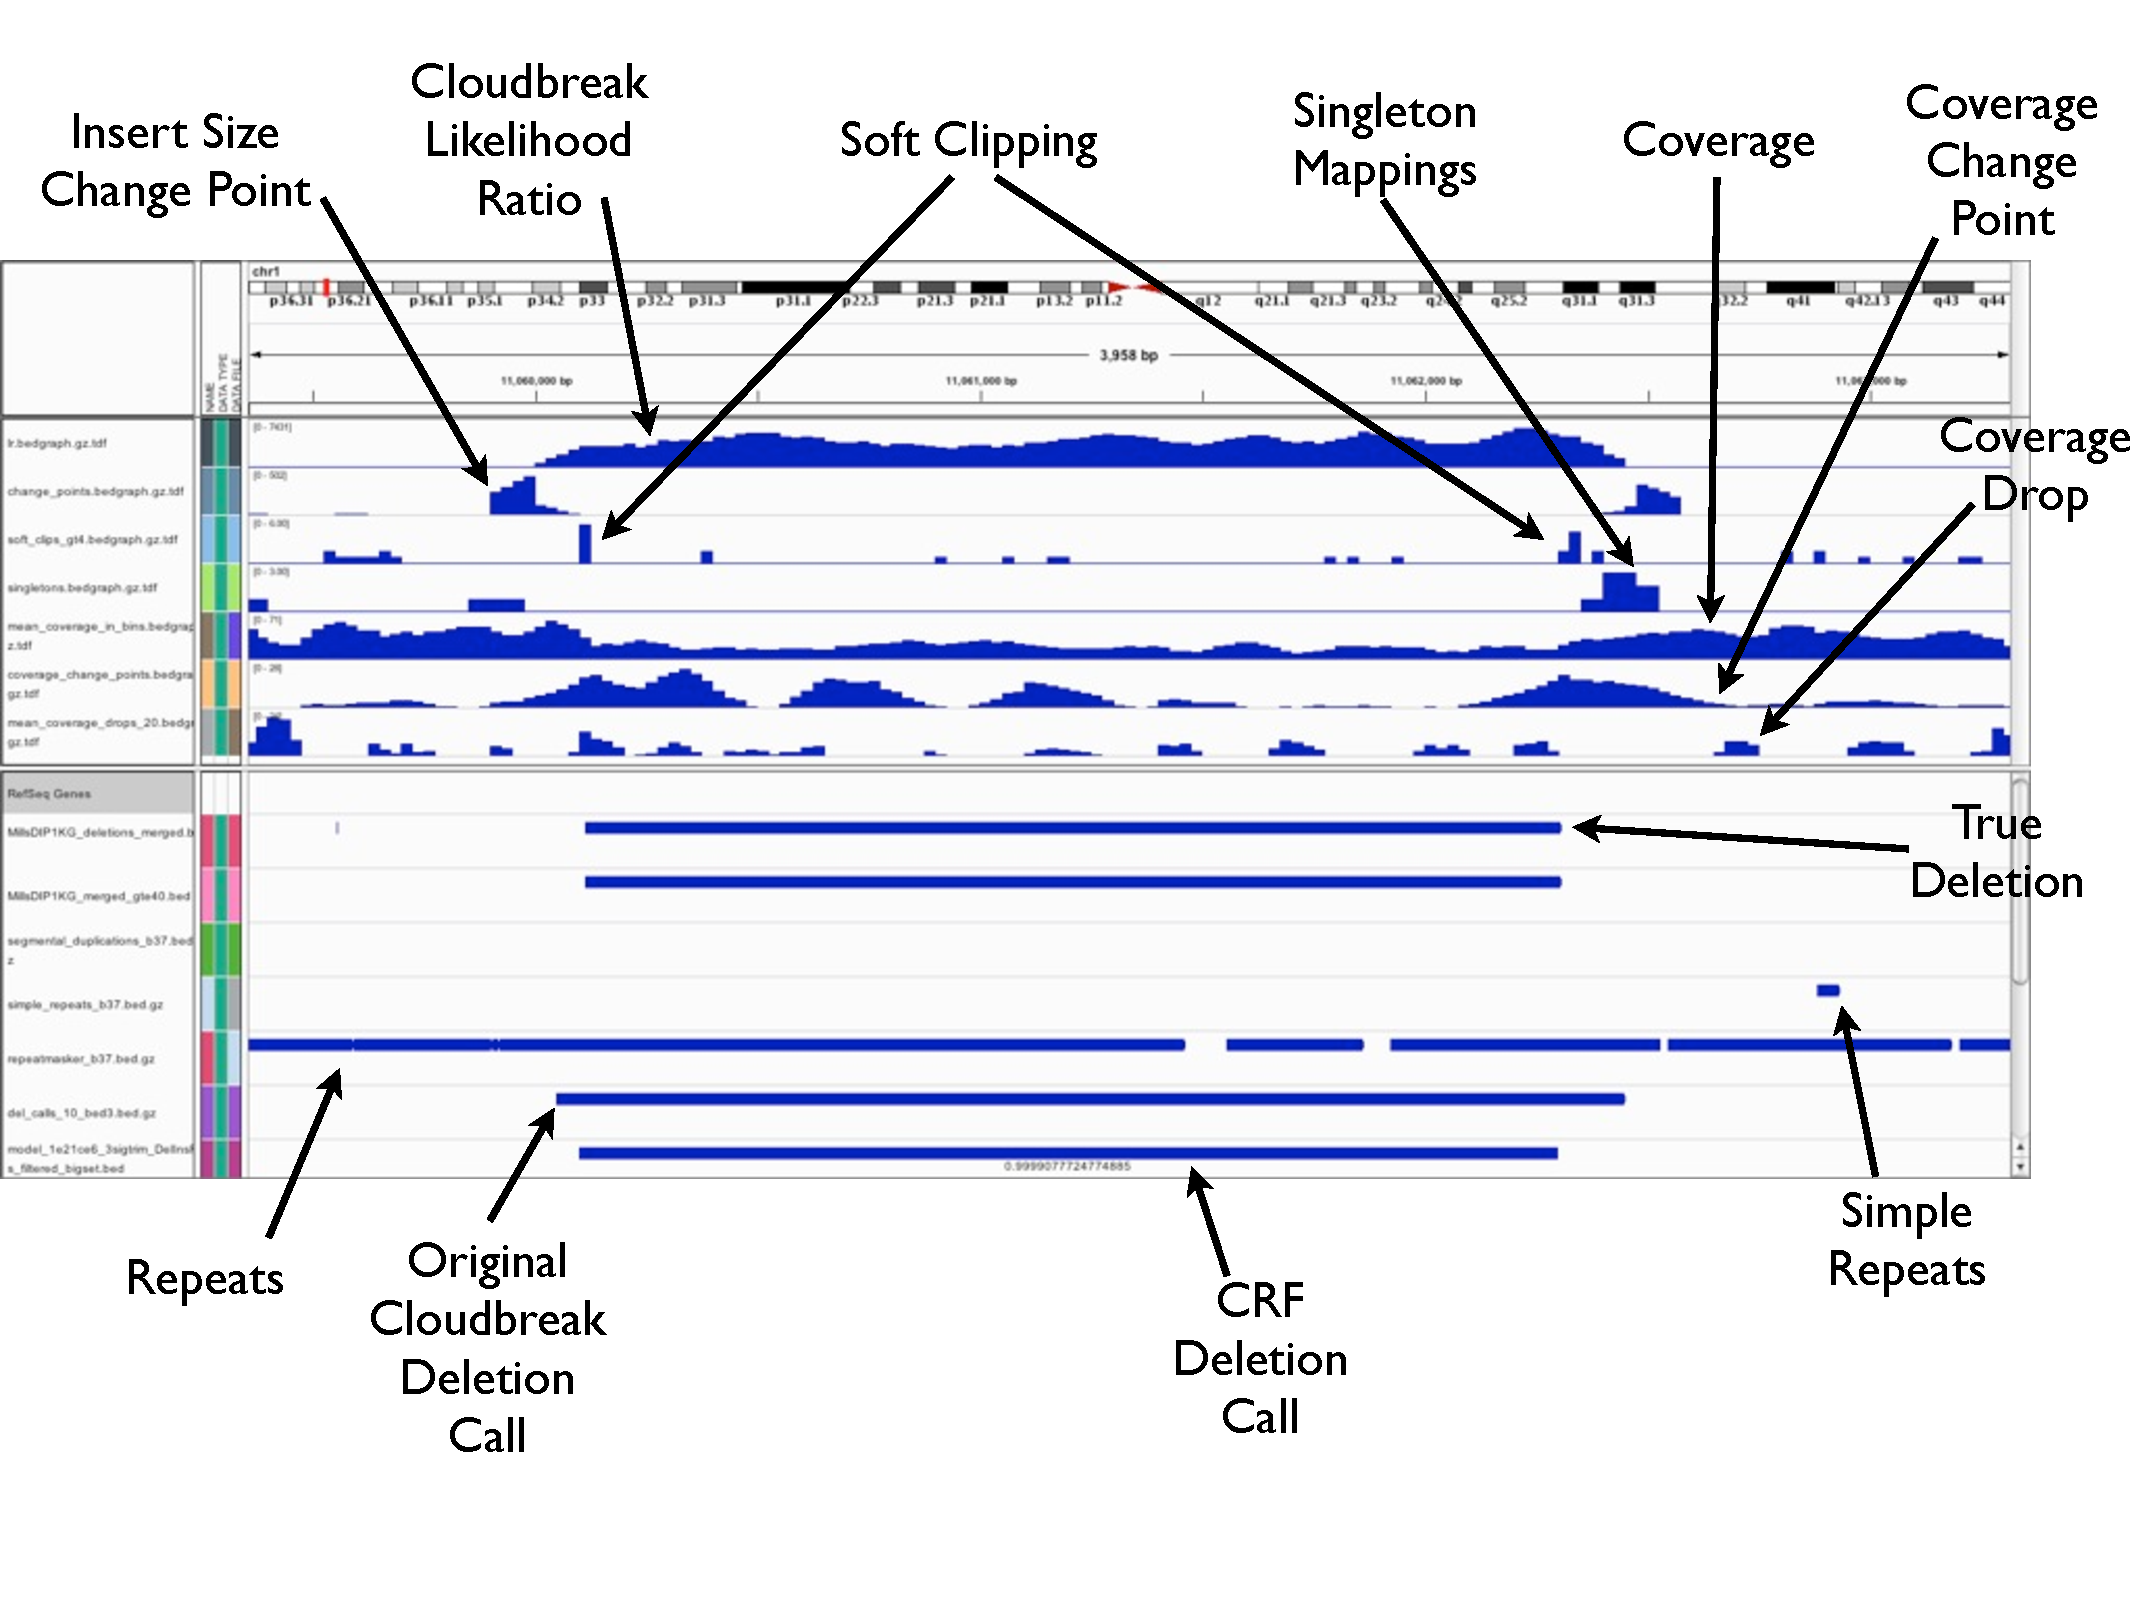
\includegraphics[width=1\textwidth]{figures/true_example_with_features.pdf}
\caption[An example deletion with features from the NA18507 data set.]{An example deletion with features from the NA18507 data set. The true deletion is shown in track 8. Features shown are in each track are: 1) Likelihood ratio of distribution of insert sizes. 2) Insert size change points. 3) Number of soft clipping events in each window. 4) Number of singleton mappings in each window. 5) Read coverage in each window. 6) Coverage change points. 7) Coverage drops. 11) Simple repeats. 12) Repeats. The original Cloudbreak call is shown in Track 13, and a call made by running inference in the CRF model is shown in Track 14.}
\label{crf_features_example}
\end{figure}

\section{Training the CRF}

As noted in Chapter~\ref{chap_cloudbreak_eval}, there are limited complete SV annotations of real data sets available. Therefore, we decided to train on simulated data. It should be noted that training on simulated data only exposes the model to one form of noise: incorrect or incomplete mappings. In real data sets, there are additional sources of noise in short read data sets, including chimeric fragments; complex structural variations, and errors in the genome reference. Therefore, any gains that can be made by training on simulated data and testing on real data are less than the possible gains that could be achieved with a more realistic training set.

To increase the number of training examples, we took the original simulation of Chromosome 2 described in Chapter~\ref{chap_cloudbreak_eval} and expanded it to a whole genome simulation. This also has the effect of increasing the possibility for mapping ambiguity, adding noise to the signal. The simulation includes all of the insertions and deletions annotated for J. Craig Venter's genome. Considering variants with a length over 40bp, there are 5,610 deletions and 6068 insertions. We simulated 30X coverage 100bp paired-end reads with an insert size of 300bp and aligned them to the reference genome using BWA, as described in Section~\ref{section_eval_data_sets}. 

We created a set of labels based on a bitmask representation of the following four states that a window could be in with respect to deletions and insertions: ``Deletion'', ``Deletion Flank'', ``Insertion'', and ``Insertion Flank''. We decided to include separate labels for flanking regions because several of the features we selected would be most likely to occur in the immediate flanks of deletion or insertion variants, such as singleton mappings, or the change point detection features. The use of a bitmasked label also means that we capture the windows that actually contain the breakpoints for each deletion or insertion under a separate label, since those windows contain both flanking sequence and variant sequence. See Figure~\ref{crf_labels} for an example of how labels are assigned to windows. This labeling scheme translates to a set of six commonly used labels: ``Outside Variant'', ``Insertion Flank'', ``Insertion Breakpoint'', ``Deletion Flank'', ``Deletion Breakpoint'', and ``Inside Deletion''. In our view, this set of labels represents the different categories of windows that are likely to have informative features. However, it is possible that other labeling schemes might prove to represent the feature space better; this would be a useful area for a more thorough future study.

\begin{figure}
\centering
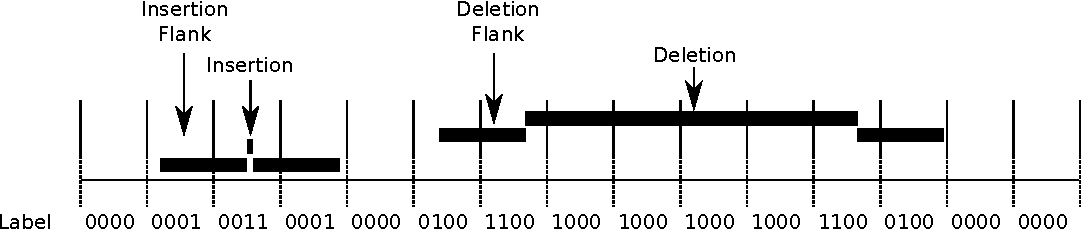
\includegraphics[width=1\textwidth]{figures/crf_labelling.pdf}
\caption[An example of the labeling scheme used for CRF model training and testing.]{An example of the labeling scheme used for CRF model training and testing. Labels are a bitmask composed of variant and flanking information. First bit: Deletion. Second bit: Deletion Flank. Third bit: Insertion. Fourth bit: Insertion Flank.}
\label{crf_labels}
\end{figure}

We also had to choose what portions of the data to train the model on, since it would be unfeasible to train on the entire reference genome, and would likely bias the model against predicting any deletions because the vast majority of the reference does not participate in a deletion variant. First, we took all of the simulated insertion and deletion variants, and added regions of 250bp with the label ``Deletion Flank'' to either side. In addition, we selected 10,774 Cloudbreak calls. Some of these overlapped with the true variants, but the others added regions to the training set which had produced false positives. We then expanded all of the 9,497 regions selected for training by first adding 400bp to either end, and then adding the length of the resulting region to both sides. This ensured that all true variants and false positives were flanked by many windows that were properly labeled ``Outside Variant''.

To train our model, we coded it in Factorie and used their implementation of the LGBFS algorithm with L2 regularization. We also experimented with other optimizers including the online AdaGrad regularized dual averaging algorithm \cite{Duchi:2011:ASM:1953048.2021068} with L1 regularization but did not see large differences in preliminary testing. A limited difference in results on the test data combined with faster training times guided our choice of LGBFS; however, exploring different optimization methods with different feature sets could still be a useful area for research.

\section{Improving Cloudbreak Calls with CRF Predictions}

For our initial implementation, we adopted the approach of rapidly identifying candidate regions using a fast tool (Cloudbreak in this instance), adding flanking regions to them, and then running the CRF model on those candidate regions to try to label the true variants. Of course, this bounds the recall of the CRF approach to the recall of the candidate regions selected by the preliminary screen, but allows for a more tractable computation than trying to label the entire genome.

For the test set, we used the same data set for individual NA18507 described in Section~\ref{section_na18507}, with 37X coverage by high-quality 100bp paired end reads with an insert size of 300bp. To choose regions to test on, we used Cloudbreak predictions for the same data set, at a low threshold to increase sensitivity. \todo{get actual number} We then created test windows to run inference on in the CRF model by again adding 200bp of flank to each side of each deletion prediction interval, and then adding the length of the interval in each direction. To conduct inference we use the Viterbi max-product belief propagation algorithm implemented in Factorie.

We then took all windows that the CRF model labeled deletions and merged contiguous blocks of windows to form intervals. For each such interval, we assign a confidence score as follows: first, for each window in the interval we calculate the sum of the likelihoods assigned to labels which indicate a deletion (i.e. have the ``Deletion'' bit set to one). We then compute the average of this window score across the entire deletion interval, giving us an overall CRF confidence in the deletion interval as a whole.

Finally, we refined the initial set of Cloudbreak deletion calls using the CRF calls according to the following rule: if a Cloudbreak deletion call and a CRF deletion call share a reciprocal overlap of at least 60\%, we consider that Cloudbreak call to be confirmed by the CRF model. By reciprocal overlap, we mean that 60\% of the length of the Cloudbreak call overlaps the CRF call, and 60\% of the CRF call overlaps the Cloudbreak call. For confirmed calls, we take the boundaries of the CRF deletion interval to be the deletion variant boundaries, and multiply the Cloudbreak deletion likelihood ratio by the CRF confidence score to get an adjusted confidence score for the confirmed call.

\section{Results}

Figure~\ref{roc_NA18507_with_crf} shows a ROC curve that compares the confirmed CRF calls with the other methods including Cloudbreak. The sensitivity of the merged CRF predictions is limited compared to the other methods. However, the updated score, which combines the Cloudbreak likelihood ratio with the CRF confidence, does provide a small improvement in discriminative power, as the true positives occur at higher thresholds than when using the unadjusted Cloudbreak score.

\begin{figure}
\centering
\includegraphics[width=\textwidth]{/Users/cwhelan/Documents/svpipeline/figures/NA18507_DELS_ROC_with_CRF.pdf}
\caption[ROC curve for CRF-confirmed Cloudbreak deletion calls.]{ROC curve showing the accuracy of Cloudbreak calls that have been verified and refined with conditional random field predictions (Cloudbreak-CRF)}
\label{roc_NA18507_with_crf}
\end{figure}

Although the CRF method provides only a limited benefit to discriminative power over the raw Cloudbreak calls, it proves to be excellent at improving the breakpoint resolution of the calls. Figure~\ref{breakpoint_resolution_NA18507_with_crf} shows the breakpoint resolution of each of the methods, as reported previously in Chapter~\ref{chap_cloudbreak_eval}, with the addition of the set of Cloudbreak calls confirmed by the CRF model. The confirmed calls have dramatically better resolution than the original Cloudbreak call set. With CRF confirmation, Cloudbreak's median difference between the true deletion length and the predicted length, 17bp, is now similar to that of DELLY-RP, which at 16bp is the best performing read-pair based method according to this metric (methods that take advantage of split-read mappings, such as DELLY-SR and Pindel, of course do better in this category). When one considers that Cloudbreak's predictions and the CRF features and labels are all based on the use of 25bp windows, it is clear that most of the time the CRF predictions are accurately identifying the window which contains the true breakpoint.

\begin{figure}
\centering
\includegraphics[width=.8\textwidth]{/Users/cwhelan/Documents/svpipeline/figures/breakpointResolutionNA18507_withCRF.pdf}
\caption[Breakpoint resolution for deletions on the NA18507 data set, including Cloudbreak CRF calls.]{Breakpoint resolution of each tool's correct deletion predictions on the NA18507 data set, including Cloudbreak calls which were verified and refined with CRF predictions (Cloudbreak-CRF)}
\label{breakpoint_resolution_NA18507_with_crf}
\end{figure}

\section{Features Selected by the CRF}

It can often be informative to examine the features that are given high scores by a machine learning technique. Table~\ref{crf_feature_selections} shows the top 25 features learned by the CRF for the window labels that correspond to ``Deletion Breakpoint'' (the windows which contain the endpoints of deleted regions) and ``Insertion''. Surprisingly, the CRF has learned a strong association between the deletion breakpoint label and the presence of simple repeats, showing how much correspondence there is between those features and the variants in the training set. As we might expect given the improvement in localizing breakpoint locations, soft clipping-related features are given high scores, particularly when they occur in conjunction with coverage drops. The mu2 feature is used heavily for both deletions and insertions. Surprisingly, the Cloudbreak likelihood ratio does not occur often in the highest scoring features. Further examination of the feature scores may allow for improvements in feature engineering to create more parsimonious and effective models.

\begin{table}
\begin{centering}
\footnotesize
\resizebox{\textwidth}{!}{
\begin{tabular}{|lr|lr|}
\hline
\multicolumn{2}{|c|}{Deletion} &	\multicolumn{2}{c|}{Insertion} \\
Feature Name & Score & Feature Name & Score \\
\hline
simpleRepeat & 0.6 & softClip > 1.0 & 0.47 \\
260 < mu2 < 340 and simpleRepeat & 0.34 & simpleRepeat & 0.41 \\
simpleRepeat neighbor & 0.34 & softClip > 3.0 & 0.39 \\
rdepth < .1 and simpleRepeat & 0.32 & 260 < mu2 < 340 and softClip > 1.0 & 0.38 \\
260 < mu2 < 340 and simpleRepeat neighbor & 0.29 & softClip > 1.0 neighbor & 0.31 \\
softClip > 1.0 and covDrop20 > 5.0 & 0.23 & softClip > 2.0 & 0.29 \\
softClip > 3.0 and covDrop20 > 5.0 & 0.2 & mu2 < 260 in region & 0.26 \\
mu2 < 260 and lr = 0 in region & 0.19 & 260 < mu2 < 340 and softClip > 3.0 & 0.25 \\
softClip > 1.0 & 0.18 & rdepth < .1 and simpleRepeat & 0.24 \\
softClip > 3.0 and covDrop20 > 10.0 & 0.17 & rdepth > 1 and simpleRepeat neighbor & 0.23 \\
softClip > 2.0 and covDrop20 > 5.0 & 0.17 & softClip > 2.0 neighbor & 0.22 \\
mu2 > 340 and simpleRepeat & 0.17 & softClip > 1.0 in region & 0.22 \\
covDrop20 > 5.0 in region & 0.17 & mu2 < 260 and simpleRepeat & 0.21 \\
changePoint > 5.0 in region & 0.16 & simpleRepeat and repeat & 0.21 \\
softClip > 2.0 and covDrop20 > 10.0 & 0.15 & singletons > 1.0 and covDrop20 > 5.0 & 0.21 \\
covChangePoint > 10.0 in region & 0.15 & softClip > 2.0 in region & 0.2 \\
softClip > 1.0 neighbor & 0.14 & softClip > 3.0 neighbor & 0.2 \\
mu2 > 340 in region & 0.14 & 260 < mu2 < 340 and softClip > 2.0 & 0.2 \\
mu2 > 340 and lr > 0.75 & 0.14 & rdepth > 1 and simpleRepeat & 0.2 \\
changePoint > 15.0 and rdepth < .5 in region & 0.14 & softClip > 1.0 and rdepth > 1 & 0.16 \\
mu2 > 340 and softClip > 1.0 & 0.13 & mu2 < 260 neighbor & 0.16 \\
softClip > 1.0 and covDrop20 > 10.0 & 0.13 & lr > 0.75 and simpleRepeat & 0.15 \\
260 < mu2 < 340 and covDrop20 > 10.0 neighbor & 0.13 & 260 < mu2 < 340 and lr = 0 in region & 0.15 \\
rdepth < .1 and covDrop20 > 5.0 neighbor & 0.13 & softClip > 1.0 and repeat & 0.15 \\
rdepth < .25 & 0.13 & changePoint > 5.0 and softClip > 3.0 & 0.14 \\
\hline
\end{tabular}
}
\caption[Most important features learned by the CRF model for deletion and insertion breakpoints.]{Most important features learned by the CRF model for deletion and insertion breakpoints. ``Neighbor'': feature occurs in neighboring window. ``In region'': feature occurs within 300bp of current window. Feature names are the same as those in Table~\ref{crf_feature_definitions}}
\end{centering}
\label{crf_feature_selections}
\end{table}

\section{Discussion}

With the CRF model presented in this chapter, we have shown that the use of local features is a useful abstraction that can enable innovative algorithmic approaches to the SV detection problem. We redefined SV detection as a sequence labeling problem, and created a framework for generating and managing local features across the genome that can integrate read pair, split read, and read depth related features, as well as features that incorporate prior knowledge such as genome annotations. Despite only training with simulated data that likely does not incorporate all of the aspects of the SV detection problem that make it difficult, we were able to generate useful predictions from our model.

Although the improvements in accuracy we achieved with the CRF model are marginal at best, it did prove to be very effective in improving Cloudbreak's breakpoint resolution, which was one of the weak points of the initial implementation of Cloudbreak as described in the previous chapters. The fact that for the majority of correctly predicted variants the CRF model was able to correctly identify the windows in which the breakpoint occurred indicates that the resolution could potentially be further improved with reductions in window size. In addition, those windows identified could be excellent targets for exhaustive split read analysis or local assembly.

Opening the door to arbitrary features potentially allows the inclusion of a variety of types of information useful for SV detection in a single unified framework. For example, other other types of genomic annotations could be very useful for detecting where the SV signals might be distorted due to sequence content. In this work we used binary features indicating the presence of repeats and segmental duplications. There are more fine-grained measures of repetitiveness and its effect on short read alignment, such as the genome mappability score \cite{Lee:2012bk} that could help to distinguish difficult regions. In addition, GC content in genomic sequence is known to have an effect on sequencing depth and copy number estimation \cite{Benjamini:2012er} and could be added as an additional feature to help correct for these biases. Another type of feature that similarly represents prior knowledge about the genome and could be incorporated into this framework is sets of predictions from different SV detection tools. The SV detection methods that have achieved the greatest overall accuracy for non-cancer domains are those that pool multiple samples from across the same population, such as Genome STRiP~\cite{Handsaker:2011ki}. The pooled signals are used to identify candidate variant regions, which are then genotyped in each sample separately in a second pass over the data. These candidate variant regions could also be used as features within an integrated machine learning technique.

Finally, the characterization of the problem as a generic sequence labeling task over arbitrary features could potentially enable the use of a variety of different statistical and machine learning techniques for the SV detection problem in addition to the CRFs explored in this chapter. For example, deep learning techniques such as sequential deep belief networks~\cite{andrew2012:sdbn} have recently been used very successfully in sequence processing tasks in speech recognition and other domains. Since it is difficult to find fully annotated training data for the SV detection problem, the fact that deep learning networks are amenable to semi-supervised training with unlabeled data \cite{weston2012} makes them a very attractive area for future research.